\documentclass[12pt]{article}
\usepackage[margin=1in]{geometry}
\usepackage{amsmath}
\usepackage{graphicx}
\usepackage{booktabs}
\usepackage{setspace}
\usepackage{caption}
\usepackage[hidelinks]{hyperref}
\usepackage{apacite}

\graphicspath{{../output/figures/}}

\title{Drug Decriminalization and College Graduation:\\
Evidence from Oregon's Measure 110}
\author{William Swartz\\
\small Department of Economics, San Diego State University\\
\small ECON 740: Seminar in Applied Economic Research\\
\small Dr.\ Penglase}
\date{December 2024}

\begin{document}
\doublespacing

\maketitle

\begin{abstract}
\noindent On February 1, 2021, Oregon became the first state in the United
States to decriminalize the possession of small quantities of all illicit
drugs under Measure 110. This unprecedented policy shift has sparked
extensive debate regarding its broader societal implications. Proponents
assert that decriminalization can reduce stigma, encourage treatment for
substance use disorders, and lessen the criminal justice burden. However,
critics caution that such measures could inadvertently increase drug use
and overdose rates. This paper constructs a synthetic Oregon, outlined by
\citeA{abadie2010synthetic}, to examine the causal impact of Measure 110 on
college graduation rates in Oregon, offering insights into how drug policy
changes may influence educational attainment.
\end{abstract}

\section{Introduction}

Does drug decriminalization reduce college graduation rates? One can
imagine two plausible scenarios in which this policy might influence
students' academic outcomes. First, for those who already use drugs,
decriminalization---alongside increased social programs addressing
substance use---may help them graduate on time by minimizing involvement
with the criminal justice system and providing improved treatment options.
Alternatively, the policy could raise overall drug use by reducing the
legal repercussions of consuming or selling illicit substances, potentially
interfering with students' ability to complete their degrees.

Historically, attending college has been considered a protective factor
against the development of substance use disorders \cite{welsh2019substance}.
However, in a study by \citeA{caldeira2009college}, nearly half of 946
college students who were followed from freshman to junior year met
criteria for at least one substance use disorder during that time.
Countless studies have shown that students who regularly use substances are
more likely to have lower GPAs, spend fewer hours studying, miss
significantly more class time, and fail to graduate on time
\cite{welsh2019substance}.

College students occupy a unique position in the drug policy debate because
they are at a critical transitional stage: many are experiencing newfound
independence, encountering academic and social pressures, and establishing
long-term habits that can influence their future well-being. This
combination of factors makes them both a vulnerable population and a group
with significant potential for positive outcomes if appropriate support
structures and policies are in place.

Moreover, college graduates typically have higher lifetime earnings, lower
unemployment rates, and are more likely to engage civically. Ensuring that
students can remain enrolled and progress toward graduation---rather than
dropping out due to legal issues, health problems, or financial strains
associated with substance use---directly contributes to the economic and
social welfare of the state. Consequently, when contemplating drug policy
reforms, the potential impact on college students' academic success and
subsequent professional opportunities becomes a vital consideration, as it
links public health interventions to broader educational and economic
goals.

Despite the importance of understanding how statewide drug policies affect
educational outcomes, there appears to be no existing research examining
Measure 110's impact on college graduation rates. This paper addresses that
gap by providing the first causal estimates of how decriminalization under
Measure 110 has influenced college completion in Oregon.

\section{Institutional Background}

Historically, U.S.\ drug policy has been largely rooted in prohibition and
strict enforcement, highlighted by the ``War on Drugs'' launched in the
1970s by President Richard Nixon, resulting in widespread criminalization
of drug-related activities and a surge in incarceration rates, often
disproportionately affecting minority groups. Throughout the 1980s and
1990s, mandatory minimum sentencing laws reinforced this punitive model,
raising concerns about its social and economic costs. By the late 20th and
early 21st centuries, policymakers and health professionals increasingly
questioned the efficacy of a purely punitive approach, pointing to issues
of addiction, public health, and prison overcrowding. In response, some
regions began experimenting with alternative frameworks---most notably
Portugal in 2001, which decriminalized all illicit drugs and channeled
resources toward treatment and harm reduction. Within the United States,
Oregon's Measure 110 represents the first comprehensive statewide effort to
decriminalize the possession of all drugs for personal use. Reflecting a
broader shift toward viewing addiction as a public health challenge rather
than a criminal one, such measures aim to reduce stigma, encourage
treatment, and ultimately address the root causes of substance abuse.

\subsection{Measure 110}

Measure 110, passed in November 2020, was a law aimed at shifting the
state's approach to substance use from criminal punishment to
health-oriented treatment. Taking effect on February 1, 2021, it reduced
penalties for possessing small amounts of certain controlled
substances---such as cocaine, heroin, methamphetamine, and ecstasy---from
felonies or misdemeanors to a new Class E violation, carrying a maximum
fine of \$100. Prior to this, possession of these substances was a Class A
criminal misdemeanor punishable in Oregon by up to a year in prison and/or
fines up to \$6{,}250. Alongside this decriminalization, the law
established Behavioral Health Resource Networks (BHRNs) aimed at providing
treatment and support, funded by redirected marijuana tax revenue and law
enforcement savings.\footnote{\url{https://olis.oregonlegislature.gov/liz/2019I1/Downloads/CommitteeMeetingDocument/227319}}
However, in 2024, drug possession was recriminalized following a campaign
by opponents of the original bill who argued the measure had failed to
address the drug crisis effectively. The Oregon legislature passed House
Bill 4002 in 2024, rolling back parts of Measure
110.\footnote{\url{https://www.opb.org/article/2024/08/29/measure-110-drug-law-deflection-posession-crime-law-oregon-recriminalization-decriminalization/}}

\section{Literature Review}

One of the primary concerns about changing drug policies is their potential
impact on youth education and development, especially given the substantial
body of public health and health economics research linking drug use to
negative academic and longer-term life outcomes. \citeA{chatterji2003illicit}
explores the relationship between adolescent drug use and educational
attainment, finding a negative association between marijuana and cocaine
use during high school and the number of years of schooling completed.
Using state-level drug policies as instruments, Chatterji's findings
suggest that substance use during critical educational years has a
significant detrimental effect on long-term educational outcomes, reducing
educational attainment by 0.2 to 0.4 years for those who used marijuana or
cocaine during high school \cite{chatterji2003illicit}. These findings are
further reinforced by \citeA{arria2015academic}, which find, via a
longitudinal cohort study and structural model, that marijuana use in
college students is associated with various negative educational outcomes
including more missed classes, lower GPA, and longer times to graduation.
Similarly, \citeA{mezza2021drug} develop a dynamic structural model that
integrates decisions on drug use, education, and labor force participation.
Their findings indicate that early drug use, particularly before age 19, is
associated with lower educational attainment and poorer labor market
outcomes later in life. This study emphasizes the potential long-term
ramifications of youth exposure to drugs, suggesting that increased access
to substances due to decriminalization could hinder educational achievement
by altering incentives to invest in schooling \cite{mezza2021drug}.

Health outcomes, particularly overdose rates, are a critical area of
concern when evaluating the impact of drug decriminalization.
\citeA{spencer2023does} examines the causal effect of Oregon's Measure 110 on
drug overdose deaths using the synthetic control method. He finds that
decriminalization led to a 23\% increase in drug overdose deaths in Oregon
during the first year post-implementation, representing 181 additional
fatalities compared to a synthetic control group constructed from other
U.S.\ states \cite{spencer2023does}. Contrasting these findings,
\citeA{zoorob2024drug} present a more nuanced analysis that controls for the
rapid introduction of fentanyl into Oregon's unregulated drug market. They
find that the surge in fatal overdoses in Oregon coincided with the influx
of fentanyl, making it difficult to attribute the increase solely to
decriminalization. After accounting for fentanyl as a potential confounder,
the effect of Measure 110 on overdose mortality becomes statistically
insignificant \cite{zoorob2024drug}. This suggests that, while the timing
of Measure 110's implementation and increased overdoses were correlated,
fentanyl's emergence may have been the primary driver, though whether
Oregon had a more drastic increase in fentanyl supply compared to other
states is unclear.

Because Measure 110 focused on harm reduction rather than punitive
measures, it is crucial to situate this policy within the broader context
of similar approaches. \citeA{maghsoudi2021drug} conduct a systematic review
of drug checking services, which aim to provide chemical analysis of drugs
to reduce harm among users. While these services have been primarily used
in European contexts, findings indicate that providing users with accurate
information about drug composition can alter consumption patterns and
reduce risky behaviors, such as the use of contaminated substances
\cite{maghsoudi2021drug}. This suggests that complementary harm reduction
strategies may be essential to mitigate the risks of decriminalization.

Although the literature consistently points to the negative effects of drug
use and remains inconclusive regarding Measure 110's impact on overdoses,
the key question is how a more lenient drug policy might influence drug use
among youth and college-age populations. In Oregon specifically,
\citeA{kerr2018oregon} find that recreational marijuana laws (RMLs) did not
significantly increase marijuana use among college students, though it is
important to note that marijuana use of college-aged students may be
endogenous to RMLs being passed. \citeA{wen2015effect}, on the other hand,
examine the effects of Medical Marijuana Laws (MMLs) on various substances.
They find that while marijuana use increased among adults post-MML, there
were no significant changes in alcohol or other drug use among youth,
indicating that perceptions and enforcement play a crucial role in shaping
policy outcomes \cite{wen2015effect}.

Despite the existing body of research on drug decriminalization and its
health and behavioral impacts, there is a gap in understanding how policies
regarding `harder' drugs may affect educational outcomes, particularly for
college students. Given the significant controversies regarding Measure 110
and the potential for increased drug exposure in communities
post-decriminalization, it is essential to explore whether these changes
have created an environment that is conducive to college completion. By
focusing on college graduation rates, this study aims to fill a critical
gap in the literature and provide insights into how policy shifts in drug
regulation may shape the educational trajectories of youth and young
adults. Understanding these dynamics is crucial for policymakers as they
navigate the complex balance between public health, safety, and educational
priorities in the context of drug policy reform.

\section{Data}

I use data from the National Center for Education Statistics (NCES),
specifically the Integrated Postsecondary Education Data System (IPEDS),
along with the American Community Survey (ACS) 1-year tables. IPEDS is a
system of 12 interrelated survey components conducted annually that gathers
data from every college, university, and technical and vocational
institution that participates in the federal student financial aid
programs. The data collections occur in fall, winter, and spring. This is
the most comprehensive postsecondary, college-inclusive data collection
available. Within the IPEDS survey, I gather institutional characteristic
data, graduation rates, and enrollment figures at the institution level
from 2012 to 2023. I then merge these with state-level economic data from
the ACS for the same period, creating a master dataset from which I
construct a synthetic Oregon.

\begin{table}[htbp]
\centering
\caption{Descriptive Statistics}
\label{tab:descriptives}
\begin{tabular}{lrrrrr}
\hline
Variable & Obs & Mean & Std. Dev. & Min & Max \\
\hline
Graduation Rate & 612 & 47.442 & 7.555 & 24.061 & 70.500 \\
Enrollment Total & 561 & 4546.794 & 1866.839 & 1883.741 & 16054.120 \\
Grad Degree & 561 & 61.489 & 36.403 & 8.300 & 93.900 \\
Unemp. Rate & 561 & 5.665 & 1.962 & 2.200 & 12.300 \\
Median Income & 561 & 62108.014 & 13282.897 & 37095.000 & 108210.000 \\
\hline
\end{tabular}

\begin{minipage}{0.95\textwidth}
\vspace{4pt}
\footnotesize
Graduation Rate and Enrollment Total come from IPEDS. Enrollment Total was
missing for 2023 since it had yet to be calculated. Grad Degree comes from
the ACS, which is the estimated percent of civilian population 25 years or
older with a professional or graduate degree. The remaining variables also
come from the ACS. All ACS estimates were missing for 2020. No missing
predictor variables are of concern when constructing synthetic Oregon since
no pre-treatment data is missing.
\end{minipage}
\end{table}

I restrict my sample to institutions offering two-year or higher degrees.
Table~\ref{tab:descriptives} shows pooled averages of my variable of
interest, college graduation rates, as well as the predictors used to
construct synthetic Oregon. Total enrollment is collected yearly at the
institutional level, which I then collapse by year and state; thus the
table shows the average total enrollment by institution by state.

Figure~\ref{fig:countrywide} shows the country-wide average graduation
rate. The graduation rate is calculated by IPEDS by cohort---full-time,
first-degree-seeking students in a particular year---that have completed
their program within 150\% of the normal time period. For a 4-year degree
this would mean that the student completes their degree within 6 years of
entering the program. For a specific year, say 2018, this is the cohort
graduating in the spring of 2019. As seen in
Figure~\ref{fig:countrywide}, the country-wide graduation rate, for all
institutions, has increased by about 5 percentage points. Even though
Measure 110 was passed in November of 2020 and did not go into effect until
February 2021, this is still our `2020' cohort.

Figure~\ref{fig:orvsus} shows Oregon's average graduation rate over time
versus the rest of the country. Figures~\ref{fig:public}
and~\ref{fig:private} split Figure~\ref{fig:orvsus} by public and private
institutions. In Oregon the graduation rate for public institutions is
lower on average than the rest of the country but is trending upwards along
with the country, while private institutions in Oregon have higher
graduation rates on average than the rest of the country but are much more
volatile and seem to be decreasing. This difference motivates opportunities
for later heterogeneity analysis. All figures show averages for both 2- and
4-year institutions.

\begin{figure}[htbp]
\centering
\caption{Country-Wide Average Graduation Rate}
\label{fig:countrywide}
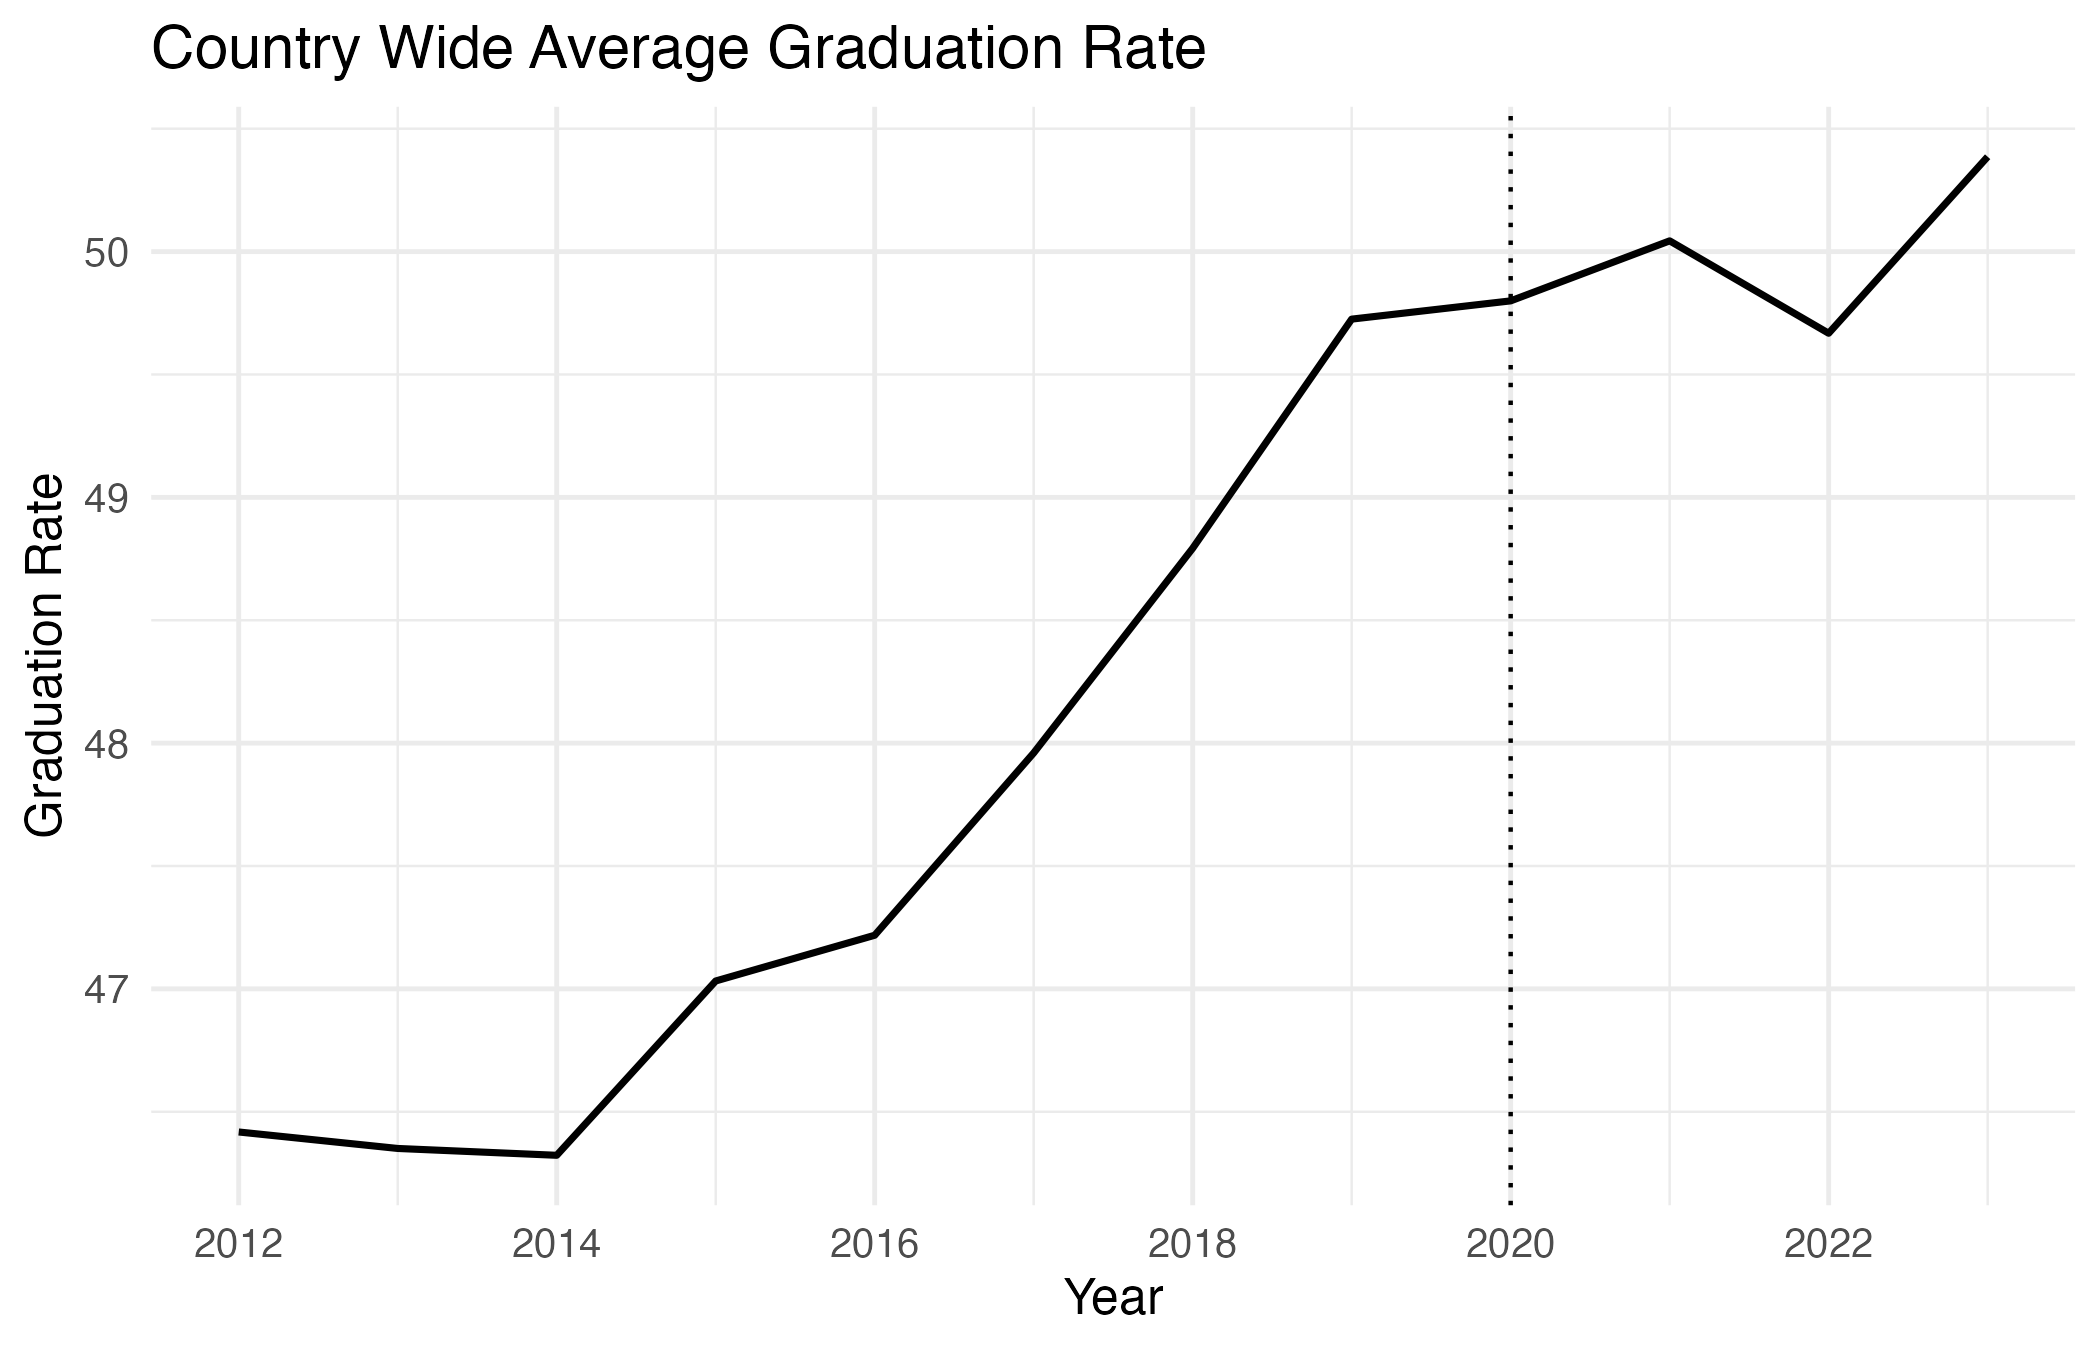
\includegraphics[width=0.85\textwidth]{fig1_countrywide_grad_rate.png}
\end{figure}

\begin{figure}[htbp]
\centering
\caption{Average Graduation Rate, Oregon vs Other States}
\label{fig:orvsus}
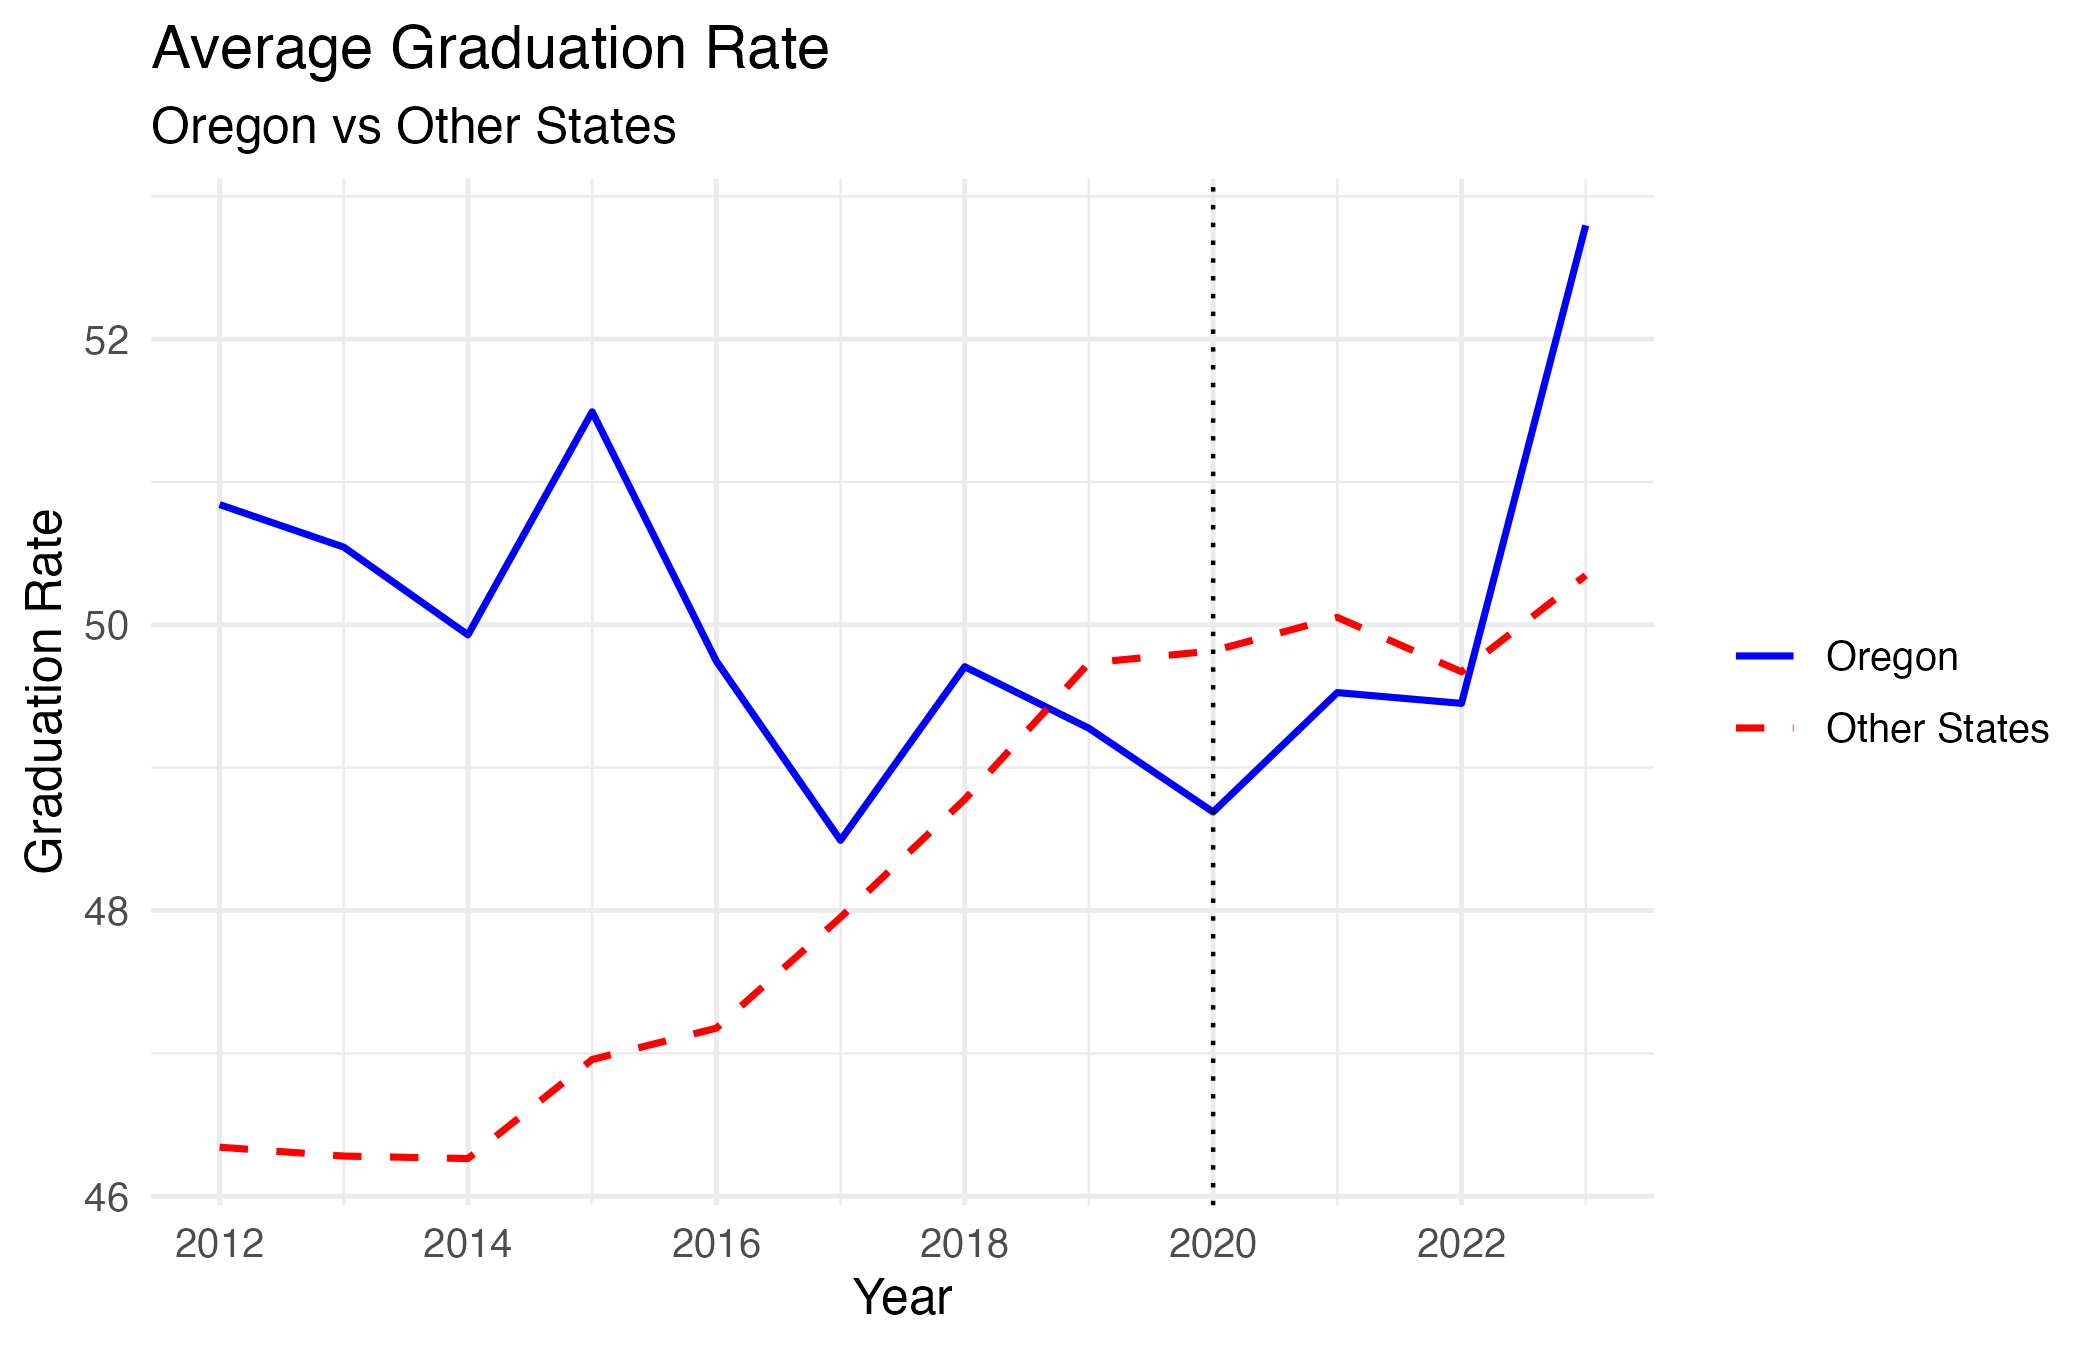
\includegraphics[width=0.85\textwidth]{fig2_oregon_vs_other.png}
\end{figure}

\begin{figure}[htbp]
\centering
\caption{Average Graduation Rate in Public Universities}
\label{fig:public}
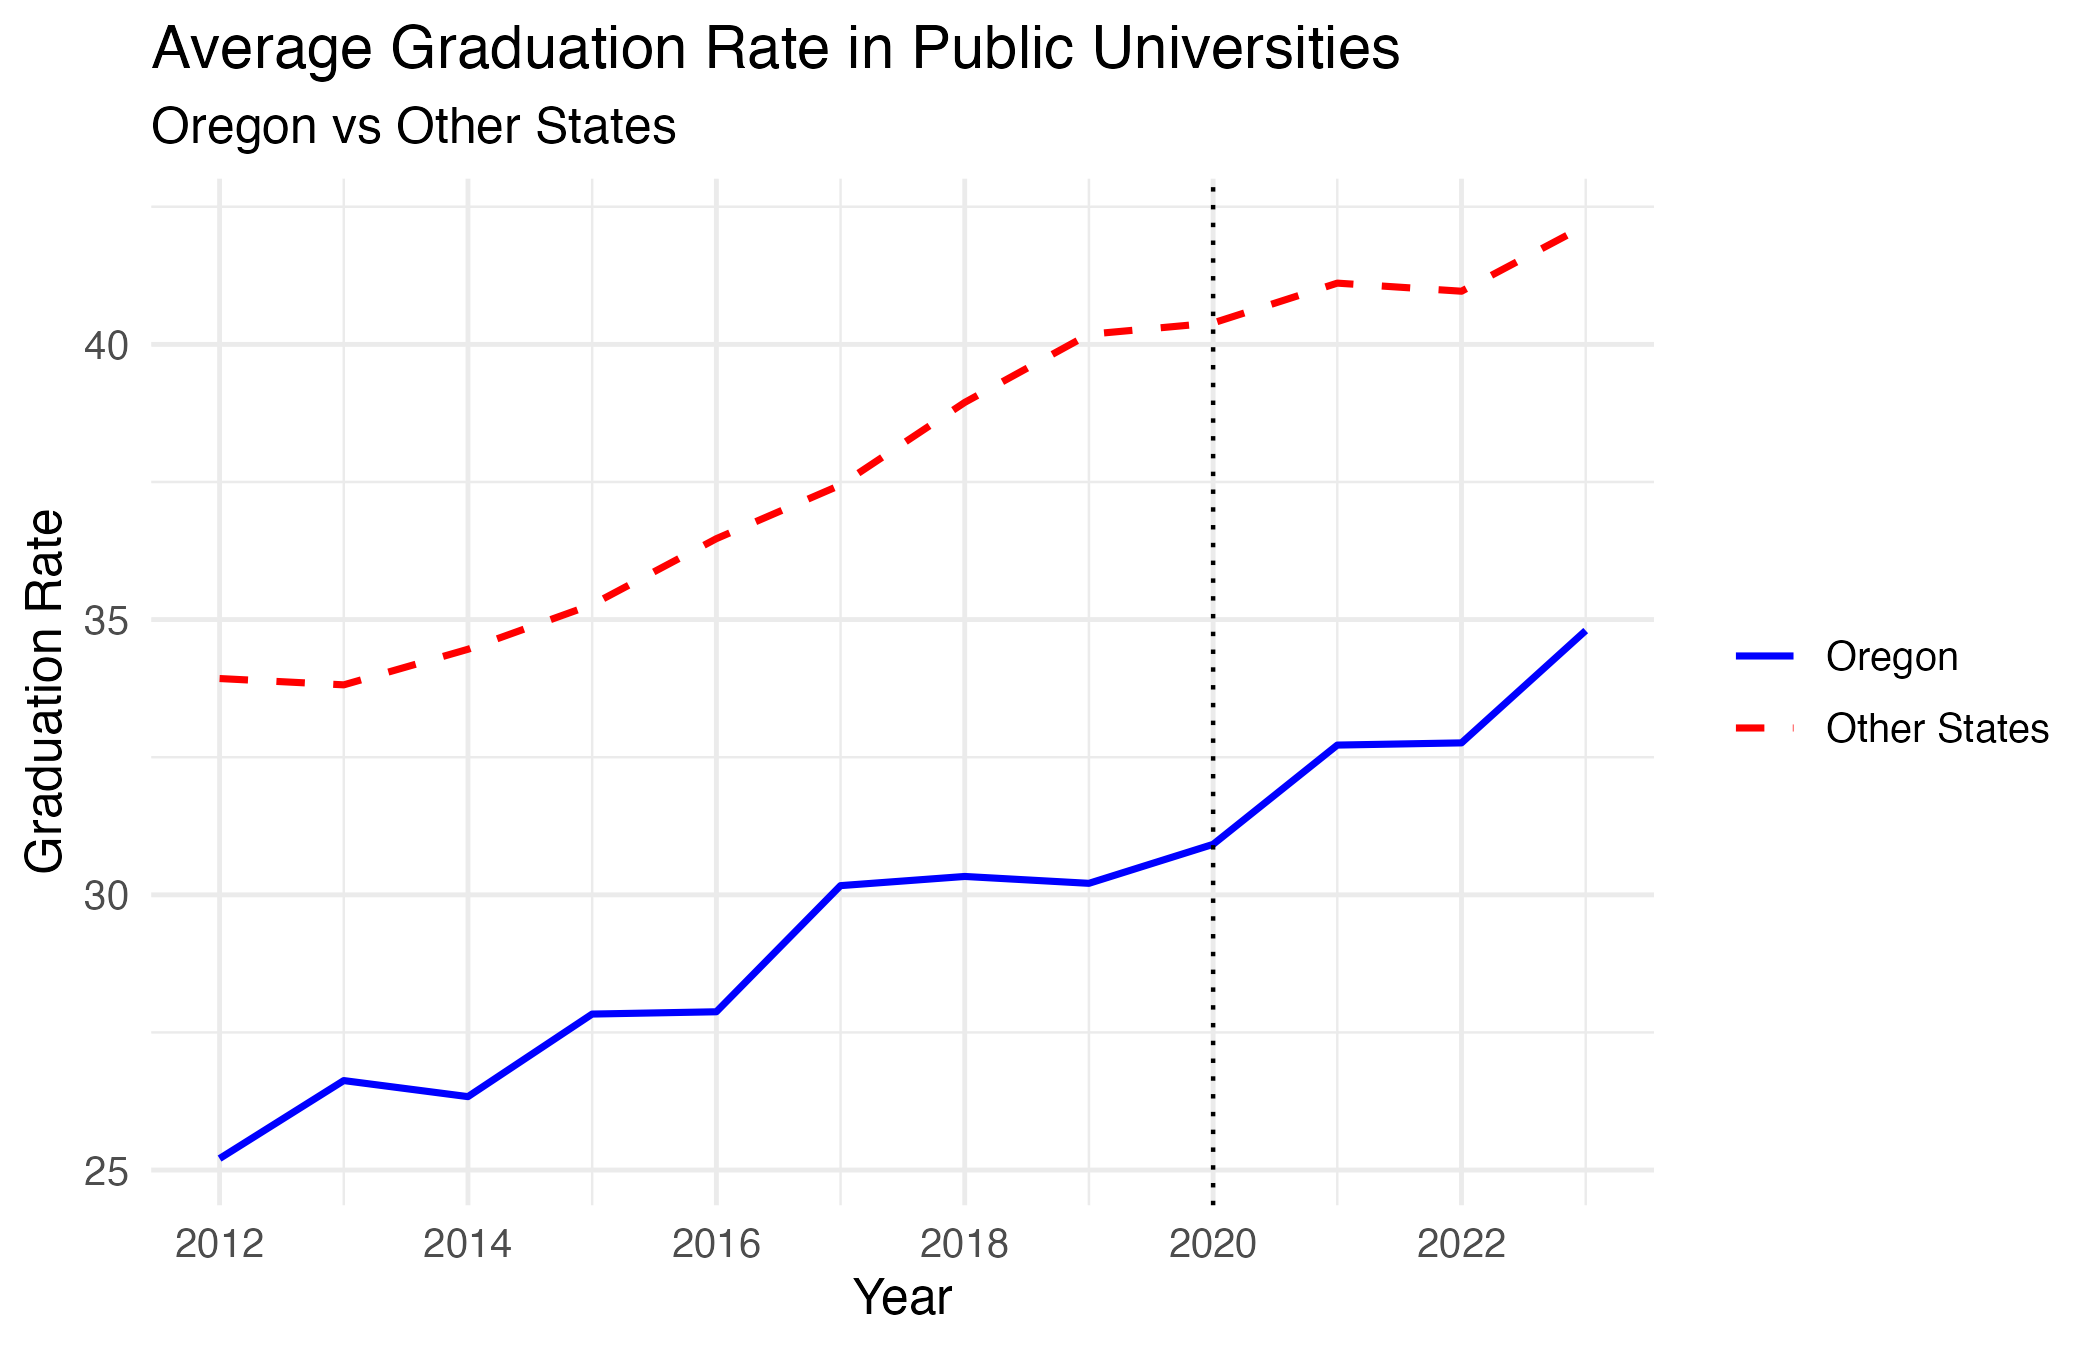
\includegraphics[width=0.85\textwidth]{fig3_public.png}
\end{figure}

\begin{figure}[htbp]
\centering
\caption{Average Graduation Rate in Private Universities}
\label{fig:private}
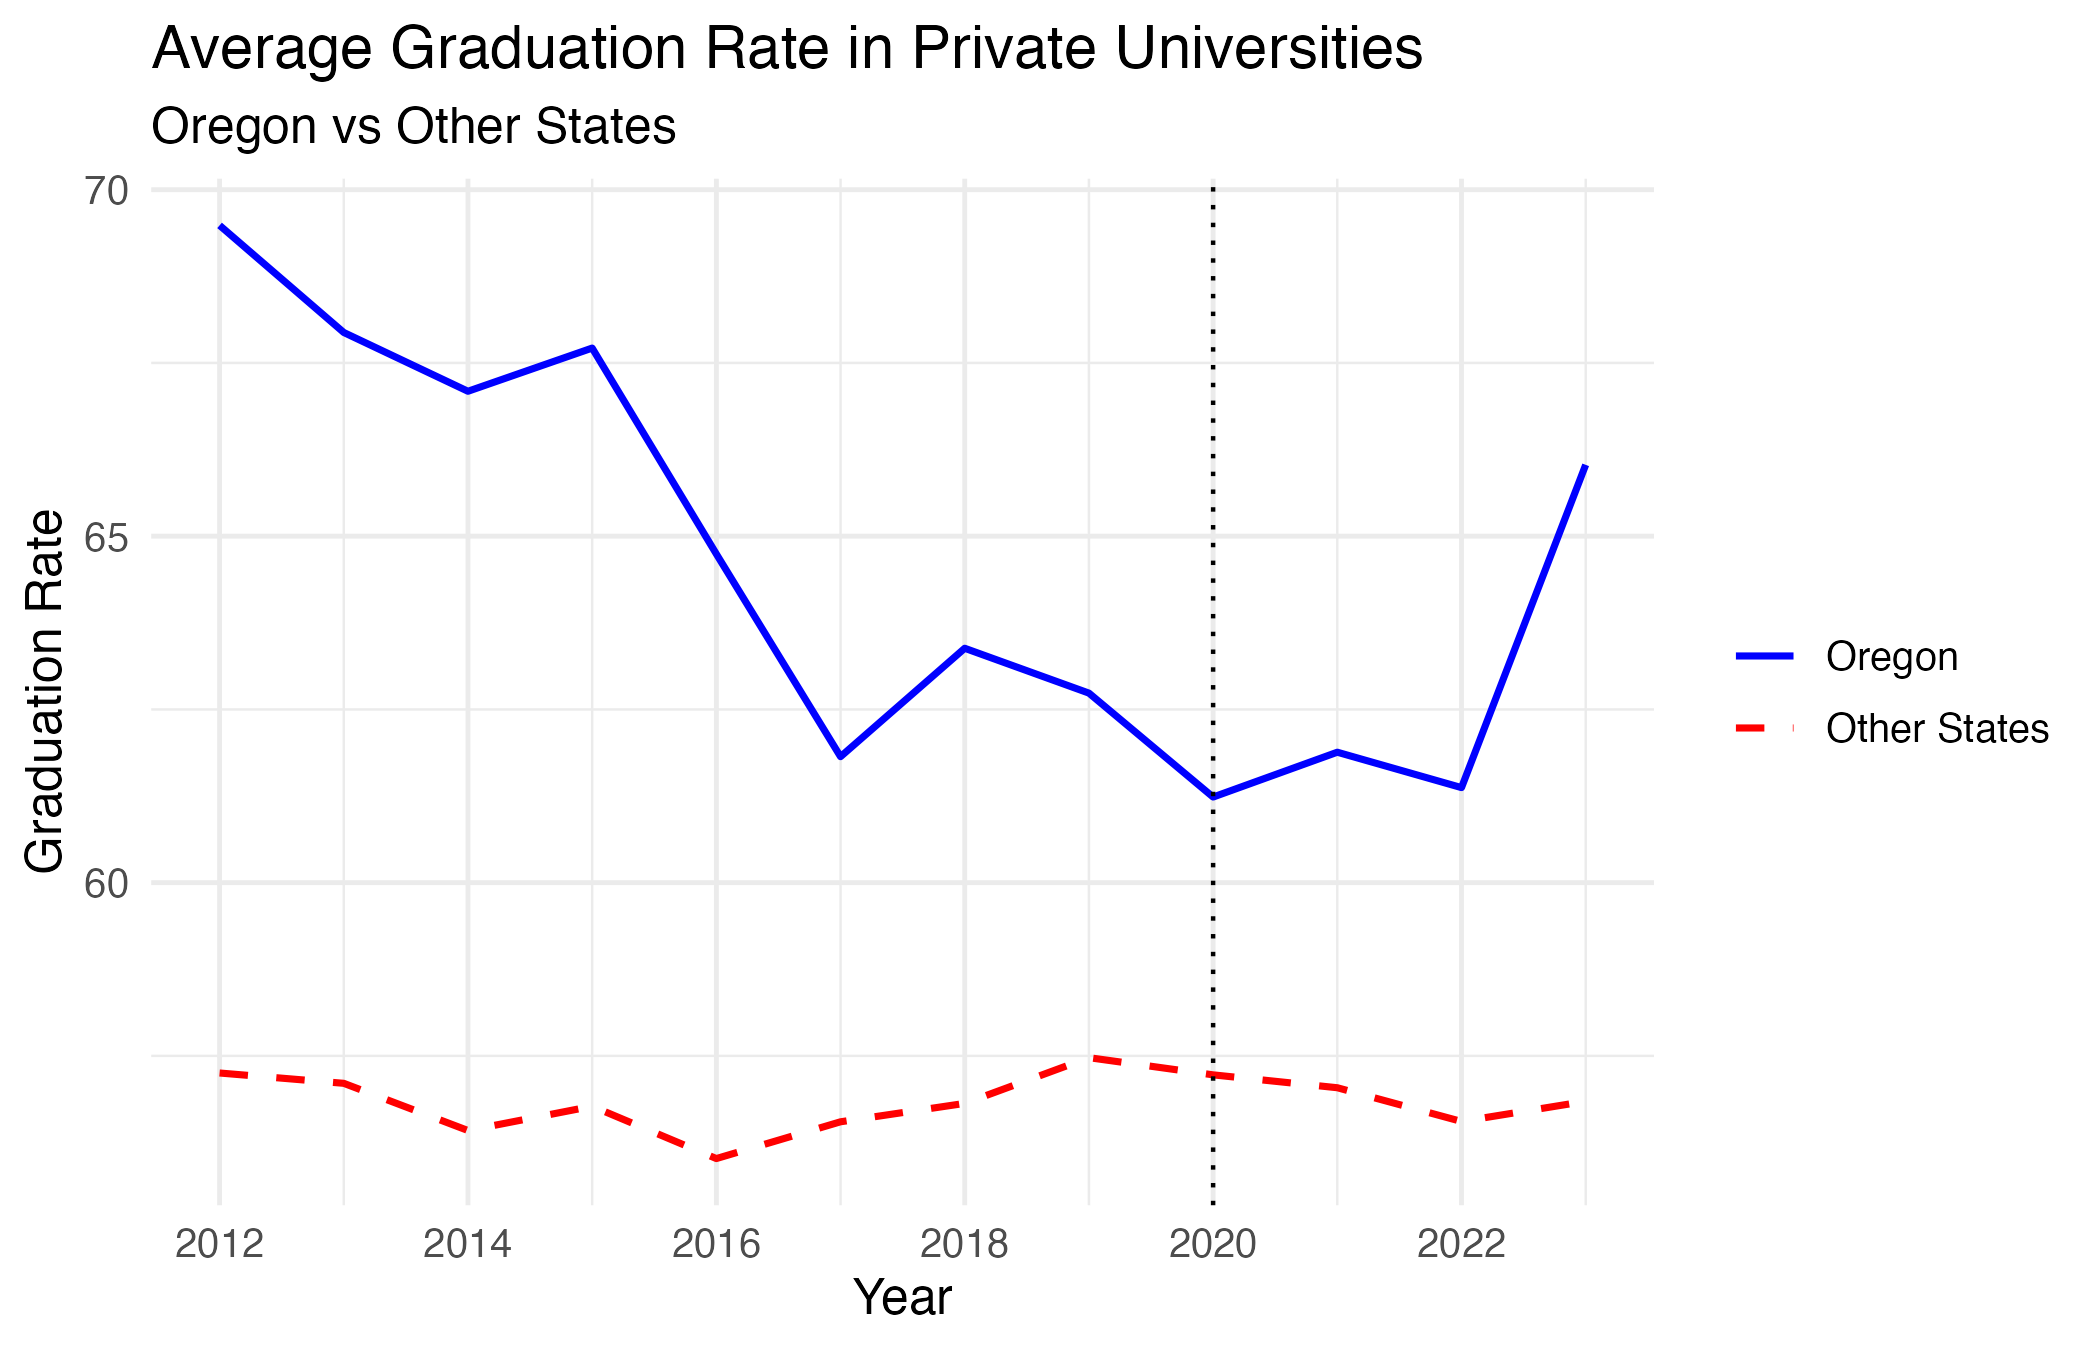
\includegraphics[width=0.85\textwidth]{fig4_private.png}
\end{figure}

\section{Econometric Strategy}

In this paper, I estimate the effect of Measure 110 on college graduation
rates using a synthetic control analysis, a method well-suited to policies
enacted in a single state. This approach involves constructing a
``synthetic'' Oregon from a donor pool consisting of the other 49 states
and Washington, D.C., thereby allowing me to measure the Average Treatment
Effect on the Treated (ATT)---that is, the difference in graduation rates
with and without Measure 110. To do this, I select a set of predictors to
weight the donor pool, minimizing the pre-treatment Mean Squared Prediction
Error (MSPE) and ensuring an optimal counterfactual.

Let $Y_{\text{Oregon},t}$ be the observed outcome, the college graduation
rate in Oregon at time $t$, and let $Y_{\text{synthetic},t}$ be the outcome
for the ``synthetic Oregon'' at the same time $t$. The synthetic unit is a
weighted average of the other states (the donor pool), with weights chosen
to match Oregon's pre-treatment characteristics. Denoting the set of donor
states as $j = 2, 3, \ldots, J$ and the corresponding optimal weights
$w_j^*$, we can write:
\begin{equation}
Y_{\text{synthetic},t} = \sum_{j=2}^{J} w_j^* \, Y_{j,t}
\end{equation}
Thus,
\begin{equation}
\text{ATT}_t = Y_{\text{Oregon},t} - Y_{\text{synthetic},t}.
\end{equation}

Despite the advantages of employing a synthetic control approach, several
challenges may arise in this setting. The effects of decriminalization on
educational outcomes may take several years to manifest; a short, in this
case three-year, post-treatment window might not fully capture Measure
110's long-term impact. Concurrent policy changes---such as alterations in
financial aid, tuition costs, or other statewide reforms---can further
complicate the isolation of Measure 110's effect, though I did not find any
evidence of this in my research. Finally, constructing a valid synthetic
counterfactual requires identifying a donor pool of states that credibly
resembles Oregon's pre-treatment trends, which can be difficult if Oregon
is an outlier or if no suitable combination of donor states exists---a
violation of the convex hull assumption.

One of the most significant threats to identification is the effect of
COVID-19 on graduation rates, which coincided with the implementation of
Measure 110. Although the pandemic affected every state, local responses,
severity, and the resulting impact on educational outcomes likely varied.
Ideally, controlling for a time fixed effect and including an interaction
term between COVID-19 severity and state would help mitigate these
confounding effects. I believe a Synthetic DiD framework may better suit
this kind of analysis in further research.

To credibly estimate a causal impact, several assumptions must hold. Most
critically, the synthetic control method relies on the assumption that, in
the absence of treatment, Oregon would have followed the same path as the
composite of donor states. This requirement necessitates strong
pre-treatment fit between Oregon and the synthetic counterpart, which is
explored in my preliminary results. Another key assumption is that Measure
110 does not significantly alter outcomes in other states, since potential
cross-border effects would compromise the donor states' validity. However,
no border states are given any weight in my donor pool. Ideally, I would
like to have removed individual institutions that border Oregon but due to
time constraints, this was not possible. I am not worried about student
migrations due to IPEDS' calculation of graduation rates being via cohort
and controlling for transfers in and out. Though even if you did believe
graduation rates were being affected by student migration because of
Measure 110, this is still a valid effect within the ATT framework.

Additionally, since I have data at the institution level and we see that
graduation rates differ across institution sectors, some heterogeneity
analysis is warranted. To do this, I subsample across sector and level,
meaning public vs private and urban vs non-urban institutions. Splitting
the sample allows the treatment effects to be different across college
types.

A final important piece of context in this analysis is that Measure 110 may
have influenced graduation rates primarily through its impact on drug use,
making any observed effect effectively a secondary or indirect policy
outcome. Ideally, I would have directly measured changes in drug use
following Measure 110 and then employed mediation analysis to determine the
extent to which drug use explained shifts in graduation rates.
Unfortunately, time constraints prevented me from conducting that
additional layer of analysis.

\section{Preliminary Results}

In this section, I present my preliminary results and discuss their
implications. I begin by reporting the main findings without subsampling
the data and then explore potential heterogeneous treatment effects by
splitting the dataset based on various institutional characteristics.

Figure~\ref{fig:synthpath} shows the synthetic control graph, comparing
Oregon's graduation rates to those of its synthetic counterpart over time.
A visual inspection reveals a strong pre-treatment fit, consistent across
all subsequent subsamples and specifications. While a na\"ive
interpretation might suggest that Measure 110 increased Oregon's graduation
rate by 4 percentage points by 2023, in-space placebo tests do not support
this conclusion. As shown in Table~\ref{tab:pooled}, the p-values for all
estimates are insignificant, and Figure~\ref{fig:placebo} further
demonstrates that this outcome is not unique.

\begin{figure}[htbp]
\centering
\caption{Oregon vs Synthetic Oregon}
\label{fig:synthpath}
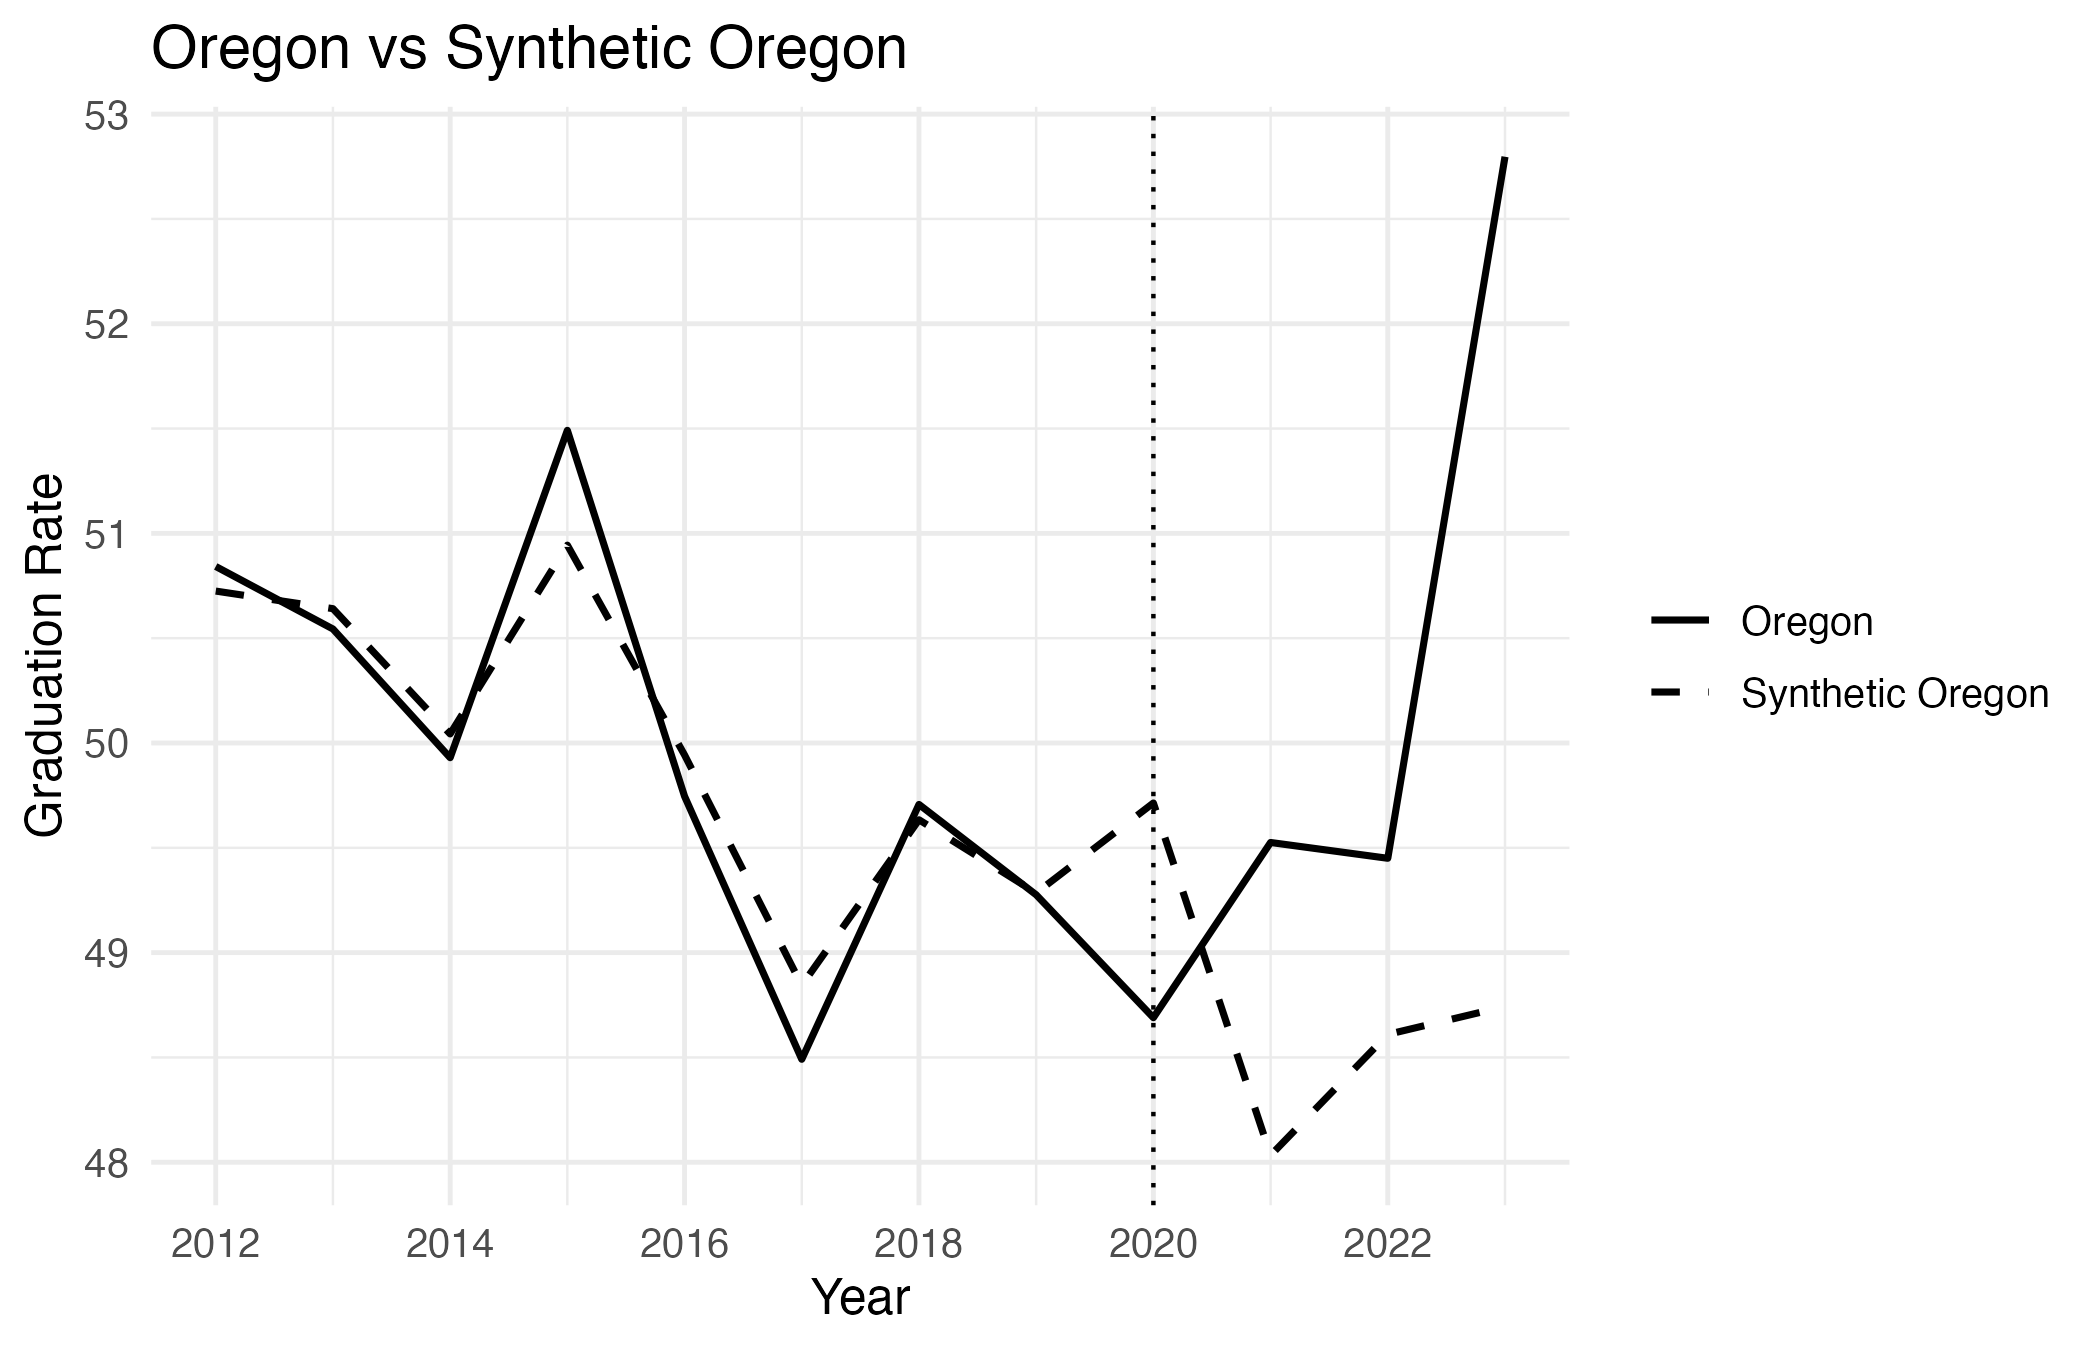
\includegraphics[width=0.85\textwidth]{fig5_synth_path.png}
\end{figure}

\begin{figure}[htbp]
\centering
\caption{Placebo Tests of Oregon vs Other States}
\label{fig:placebo}
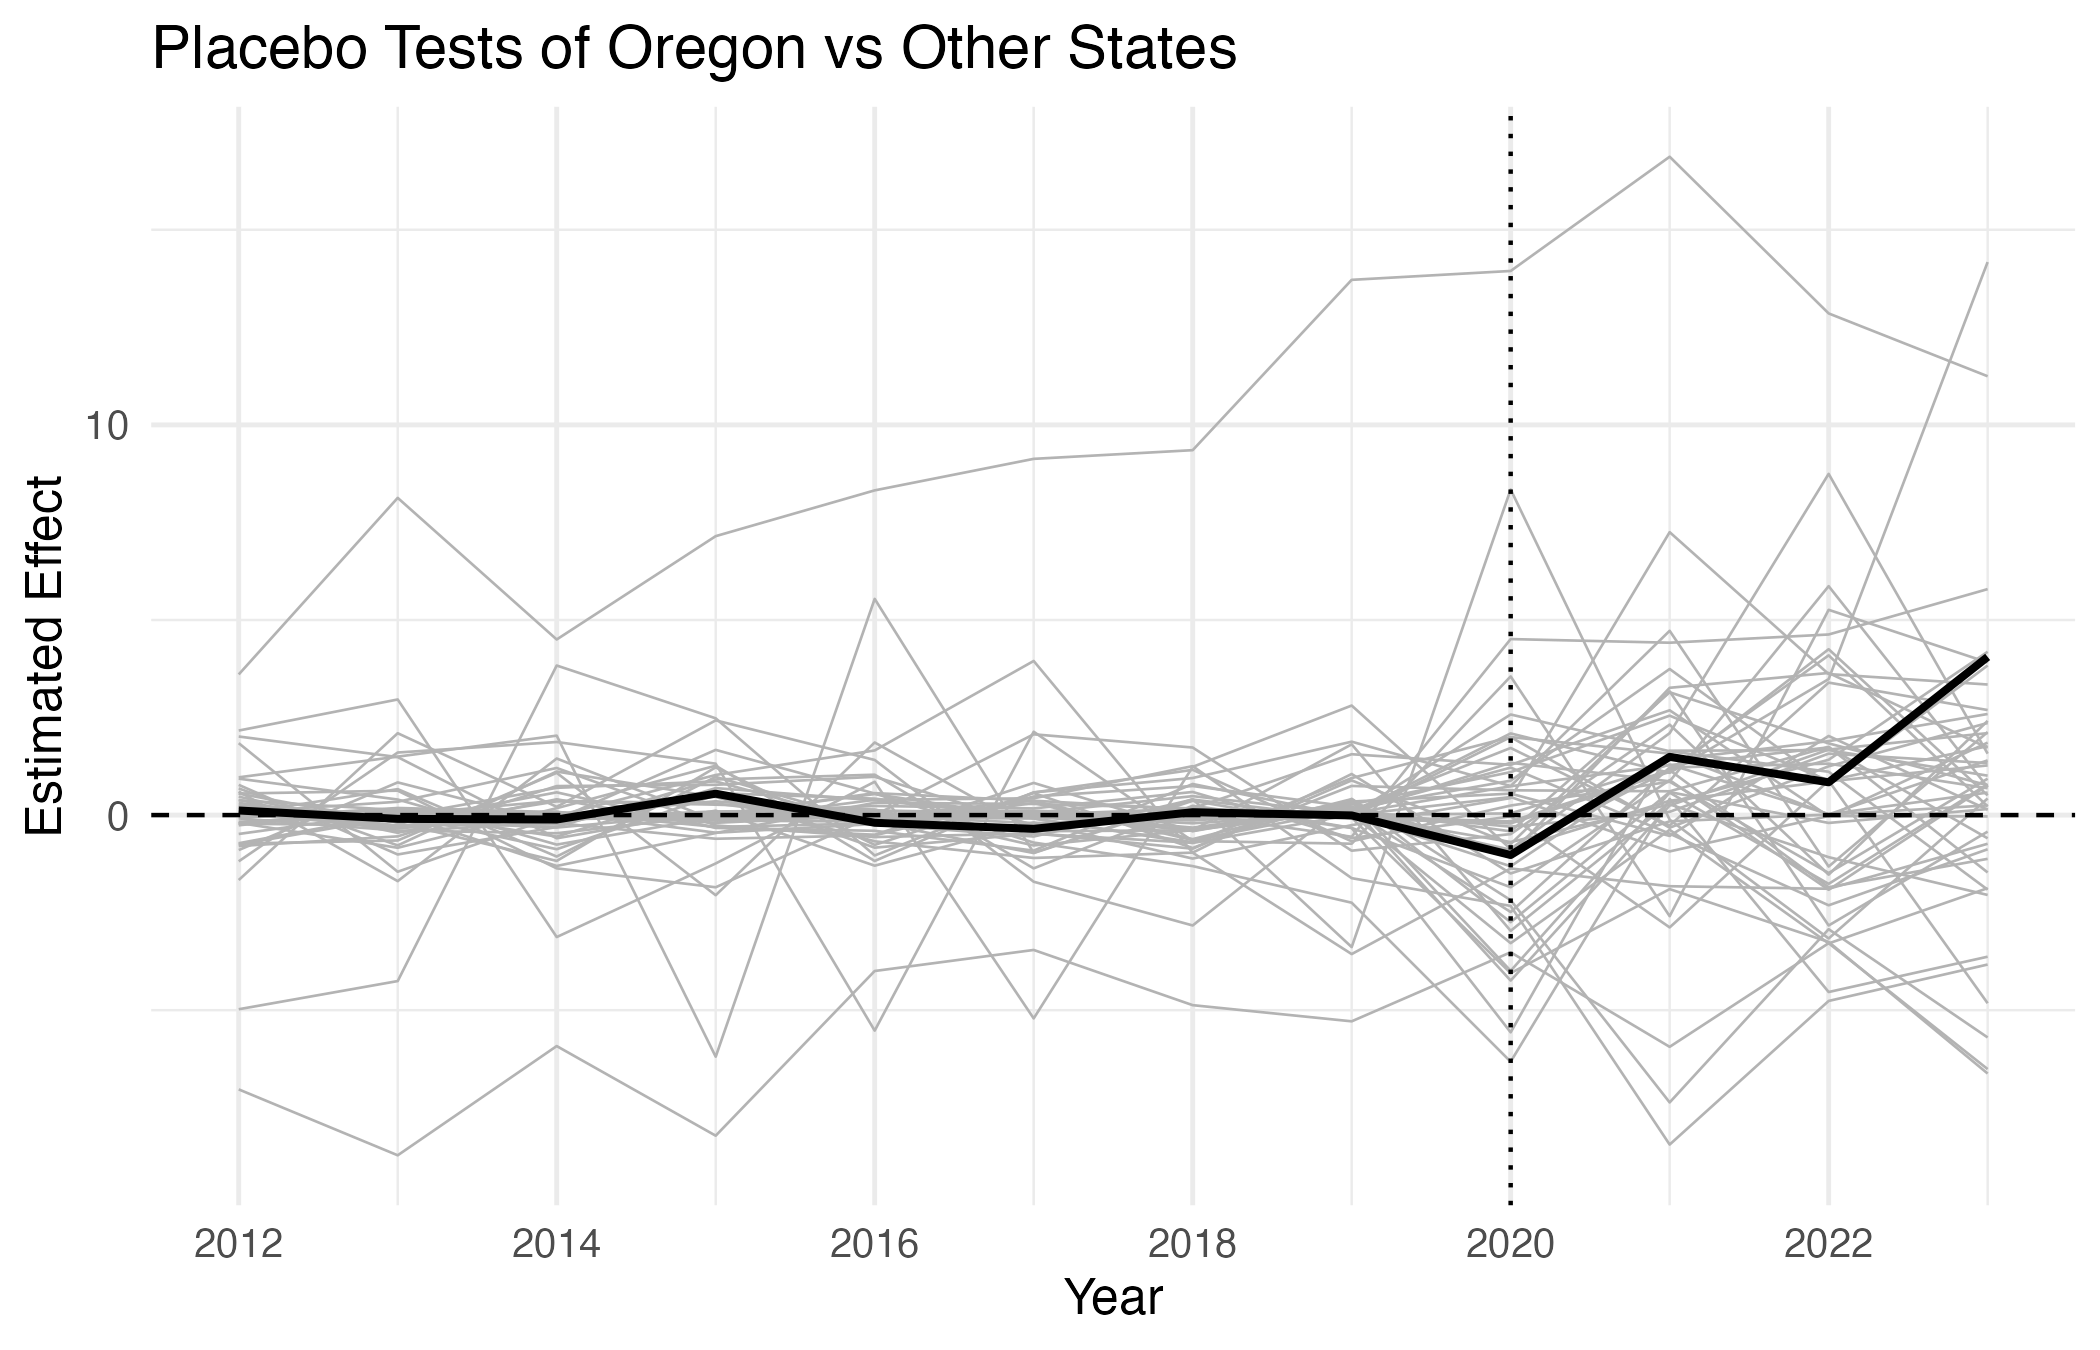
\includegraphics[width=0.85\textwidth]{fig6_placebo.png}
\end{figure}

\begin{table}[htbp]
\centering
\caption{ATTs and Associated P-Values, All Institutions}
\label{tab:pooled}
\begin{tabular}{lccc}
\hline
 & Estimate & P-value & Standardized P-value \\
\hline
2020 & -1.024 & 0.58 & 0.420 \\
2021 & 1.492 & 0.44 & 0.320 \\
2022 & 0.840 & 0.86 & 0.520 \\
2023 & 4.053 & 0.16 & 0.160 \\
\hline
\end{tabular}

\begin{minipage}{0.8\textwidth}
\vspace{4pt}
\footnotesize
All institutions. ATTs and p-values constructed via in-space placebo tests
(R implementation of \texttt{synth\_runner}).
\end{minipage}
\end{table}

For the rest of this section I show just the tables, like
Table~\ref{tab:pooled}, for the remaining subsamples, none of which result
in any significant effects.

\begin{table}[htbp]
\centering
\caption{ATTs and Associated P-Values, Public Institutions}
\label{tab:public}
\begin{tabular}{lccc}
\hline
 & Estimate & P-value & Standardized P-value \\
\hline
2020 & -0.149 & 0.94 & 0.940 \\
2021 & 1.136 & 0.60 & 0.460 \\
2022 & 0.083 & 0.92 & 0.880 \\
2023 & 3.001 & 0.26 & 0.320 \\
\hline
\end{tabular}

\begin{minipage}{0.8\textwidth}
\vspace{4pt}
\footnotesize
Public institutions. ATTs and p-values constructed via in-space placebo
tests (R implementation of \texttt{synth\_runner}).
\end{minipage}
\end{table}

\begin{table}[htbp]
\centering
\caption{ATTs and Associated P-Values, Private Institutions}
\label{tab:private}
\begin{tabular}{lccc}
\hline
 & Estimate & P-value & Standardized P-value \\
\hline
2020 & -1.449 & 0.72 & 0.620 \\
2021 & 1.741 & 0.64 & 0.620 \\
2022 & 1.595 & 0.60 & 0.560 \\
2023 & 7.709 & 0.10 & 0.140 \\
\hline
\end{tabular}

\begin{minipage}{0.8\textwidth}
\vspace{4pt}
\footnotesize
Private institutions. ATTs and p-values constructed via in-space placebo
tests (R implementation of \texttt{synth\_runner}).
\end{minipage}
\end{table}

\begin{table}[htbp]
\centering
\caption{ATTs and Associated P-Values, Urban Institutions}
\label{tab:urban}
\begin{tabular}{lccc}
\hline
 & Estimate & P-value & Standardized P-value \\
\hline
2020 & -0.987 & 0.84 & 0.800 \\
2021 & -1.742 & 0.58 & 0.620 \\
2022 & -1.398 & 0.68 & 0.640 \\
2023 & 3.870 & 0.44 & 0.520 \\
\hline
\end{tabular}

\begin{minipage}{0.8\textwidth}
\vspace{4pt}
\footnotesize
Urban institutions. ATTs and p-values constructed via in-space placebo
tests (R implementation of \texttt{synth\_runner}).
\end{minipage}
\end{table}

\section{Conclusion}

I did not find any evidence that Measure 110 influenced college graduation
rates under any of the specifications or subsamples tested. Future research
may be warranted to first determine whether Measure 110 affects college
students' drug use, as that could provide a clearer link between the policy
and educational outcomes. However, based solely on the results here, there
is no indication that Measure 110 has a significant impact on graduation
rates. Exploring further subsampling and heterogeneity analyses across
different demographic groups and institutional characteristics could be a
promising direction for additional study.

\bibliographystyle{apacite}
\bibliography{references}

\end{document}
